\section{Datenstruktur der Firmen und des Firmenkonglomerates}
Jede Firma wird in meiner Implementierung durch ein Objekt abgebildet, welches neben einer ID und dem Wert als Double auch eine Liste über alle unmittelbaren Nebenbedingungen enthält. Ich habe mich somit für die gängige Implementierung der Graphstruktur als Adjazenzliste entschiden. Da die einzige Operation auf dem Graphen eine Tiefensuche ist, ist die Adjazenzliste die geeigneteste Implementierung.\footnote{vgl. Sedgewick, Algorithmen: S. 563 (Deutsche Übersetzung der 4. Auflage)}

Das Firmenkonglomerat speichert alle Firmen des Konglomerates als Array nach Firmen-ID indiziert. Darüber hinaus speichert es die Nebenbedingungsmengen zu jeder Firma wie auch die Information, welche Nebenbedingungsmengen ausschließlich positivwertige Firmen beinhalten, in weiteren Arrays ab. Die Konglomeratsklasse verfügt über Methoden zur Bestimmung der Nebenbedingungsmengen und der idealen Teilmenge.

\section{Bestimmen der Nebenbedingungen jeder Firma}
Die Menge aller Nebenbedingungen eines Feldes \(A\) ist äquivalent zu den besuchten Knoten einer Tiefensuche von diesem Feld \(A\) aus. Schließlich ist es das Funktionsprinzip einer Tiefensuche, alle Felder abzusuchen, zu denen ein Pfad von einem Feld führt. Eine Tiefensuche funktioniert, indem zunächst alle angrenzenden Knoten des Feldes \(A\) (die Nebenbedingungen) auf einen Stapel\footnote{Stack, Stapel, Kellerspeicher: Linearere Datenstruktur, das zuletzt abgespeicherte Objekt ist das zuerst ausgegebene Objekt (FIFO-Prinzip)} gespeichert werden.
Außerdem wird \(A\) der Besucht-Menge hinzugefügt. Alle Felder auf dem Stapel werden nun ebenfalls der Menge hinzugefügt. Die an diese Felder angrenzenden Felder werden widerum auf den Stapel gelegt, sodenn sie nicht schon in der Besucht-Menge liegen. So wird jedes Feld, zu dem von \(A\) ein Pfad führt, aufgelistet. Diese Besucht-Menge entspricht daher der Teilmenge von \(G\), die beim Kauf von \(A\) mitgekauft werden muss. Der Algorithmus kann sich nicht in einem Zyklus verfangen, da wiederholte Besuche eines Feldes aufgrund der Besucht-Menge verhindert werden. Die Nebenbedingungsmengen für jede Firma speichere ich in einem Array der Firmenkonglomeratsklasse.

Bei der Tiefensuche ermittele ich außerdem, ob eine negativwertige Firma unter den angrenzenden Firmen liegt. Dies ist, wie in der Lösungsidee beschrieben, zur Beschleunigung des Algorithmusses relevant. Ob eine negativwertige Firma in der Ergebnismenge enthalten ist, speichere ich einem Array.

Zentral für die Umsetzung der Lösungsidee ist die effiziente Abbildung der Besucht-Menge im Speicher. Naheliegend ist die Verwendung der Klasse Set, jedoch ist diese bei genauerer Betrachtung nicht optimal. Sinnvoller ist die Verwendung eines BitSets. Ein BitSet besteht in Java aus einer Abfolge von \(n\) binären Bits. Für unsere Anwendung wird für jede Firma ein Bit benötigt.
Steht das Bit \textit{n} auf 1, befindet sich die \textit{n}te Firma in der durch das BitSet repräsentierte Menge. Steht es auf 0, befindet sich die Firma nicht in der Menge.
Die Verknüpfung zweier Mengen entspricht bei einem Bitset einer nicht-exklusive ODER-Verbindung (siehe Tabelle \ref{tab:veroder}.
Das BitSet ist besser geeignet, da anstatt der jeweiligen Firmennummern als 32bit-Integer nur einzelne Bits abgespeichert werden müssen. Außerdem gelingt die Vereinigung zweier Firmen schneller, da keine Zahlen verglichen werden müssen. Ein weiterer Vorteil des BitSets ist, dass es wahlfreien Zugriff unterstützt, während ein Set in der Standardimplementierung nur über Iteratoren auslesbar ist.
\begin{table}
	\centering
    \begin{tabular}{l|ccccccccc}
    Firma 	& A & B & C & D & E & F & I & R & Z \\ \hline
    \(M_A\)	& 1 & 0 & 1 & 1 & 0 & 0 & 0 & 1 & 0 \\
    \(M_B\)	& 0 & 1 & 0 & 0 & 1 & 0 & 1 & 1 & 0 \\ \hhline{=|*{9}{=}}
    ODER 	& 1 & 1 & 1 & 1 & 1 & 0 & 1 & 1 & 0 \\
    \end{tabular}
    \caption {Vereinigung entspricht ODER}
    \label{tab:veroder}
\end{table}

\section{Aufstellen des Baumes}
Für die Repräsentation des Baumes habe ich aufgrund der spezifischen Anforderungen des Algoritmusses einen neue Datenstruktur, eine \textit{BufferedMap}, implementiert. Diese ist aus vielerlei Gründen besser geeignet als ein Array oder eine auf Referenzen basierende Struktur.
Eine BufferedMap besteht aus einer Map, auf das nur lesend zugegeriffen werden kann, und einem Puffer, auf den wiederum nur schreibend zugegriffen werden kann. Neue Einträge werden zunächst auf den Puffer geschrieben und zu einem späteren Zeitpunkt gesammelt der Map hinzugefügt. Der Puffer ist als Stack implementiert. Die Map hat als Schlüssel eine Menge, also ein BitSet, und als Wert den Wert in Euro dieser Menge.

Ein Vorteil dieser Datenstruktur ist, dass auf die Map geschrieben werden kann, während gleichzeitig über die Map iteriert wird. Der Iterator der Map bleibt stabil, die während der Iteration geschriebenen Daten werden während der weiteren Iteration nicht ausgelesen. Erst nach der Iteration werden sie dem Set über den gesammelten Schreibvorgang hinzugefügt.

Außerdem werden dank der durch die Map gegebene Eindeutigkeit der Keys nicht \(2^V\) Blätter aufgestellt, da viele Blätter des Baumes nach Betrachtung von Nebenbedingungen äquivalent sind. Im Beispiel aus Abbildung \ref{abb:vereinigung} sind beispielsweise die Mengen von den Kaufwünschen \(B\) und \(B, E\) nach Einbeziehung der Nebenbedingungen äquivalent,da \(B\) \(E\) als Nebenbedingung hat. Solche Dopplungen werden von der Map durch Vergleich der HashCodes automatisch herausgefiltert.

In einem ersten Schritt fasse ich alle Nebenbedingungsmengen, die während der Tiefensuche als "`Win-Win-Menge"' identifiziert wurden, zu eben dieser "`Win-Win-Menge"' zusammen. Diese Menge, wie oben beschrieben repräsentiert durch ein BitSet, füge ich nun als erstes Element der BufferedMap hinzu.
Darüber hinaus speichere ich in zwei seperaten Variablen den Wert und alle Firmen der bisher besten der "`Win-Win-Menge"' initialisiert. Diese Variablen dienen als Speicher für den bis dato besten gefundene Kauf. Sobald der Baum komplett aufgebaut ist, findet sich in diesen Variablen der beste Kauf des Konglomerates.

Danach ermittele ich die Liste pm, also den Firmen die Teil des Kaufwünsches für den besten Kauf sein könnten. Dies geschieht, indem ich alle Nebenbedingungsmengen, deren Ursprungsfirma einen positiven Wert hat und die noch nicht in der "`Win-Win-Menge"' enthalten sind, in diese Liste hereinkopiere. Die Liste ist als HashSet implementiert um mögliche Doppelungen herauszufiltern. Nun führe ich folgende Logik für alle Nebenbedingungsmengen aus der Liste pm aus:
Ich füge der BufferedMap alle Kombinationen aus den bisher errechneten Käufen und einer Nebenbedingungsmenge aus pm hinzu. Die geschieht, indem ich über die gesamte Map iteriere und jeden Mapeintrag mit der Nebenbegingungsmenge verknüpfe. Den daraus resultierenden Eintrag lege ich auf den Puffer, da die gleich Firma ja nicht zweimal in einer Eintrag kombiniert werden kann. Wenn alle Mengen verknüpft sind, leere ich den Puffer und fahre mit der nächsten Nebenbedingungsmenge fort. Damit erhalte ich alle Blätter des Baumes (s. Illustration TODO). Falls dabei eine Menge gefunden wird, deren Wert höher als das bisherige Maximum ist, speichere ich diese Menge und ihren Wert in den entsprechenden Maximumsvariablen. So finde ich mit absoluter Sicherheit die günstigste Kombination. Durch diese Implemenentation des Baumes verliere ich alle Generationen bis auf die letzte. Da aber alle Käufe in den Blättern vorhanden sind, geht keine relevante Information verloren. Den Zuwachs der Map von Schleifendurchlauf zu Schleifendurchlauf habe ich in Abbildung \ref{abb:map} skizziert.

\begin{figure}[!h]
	\centering
	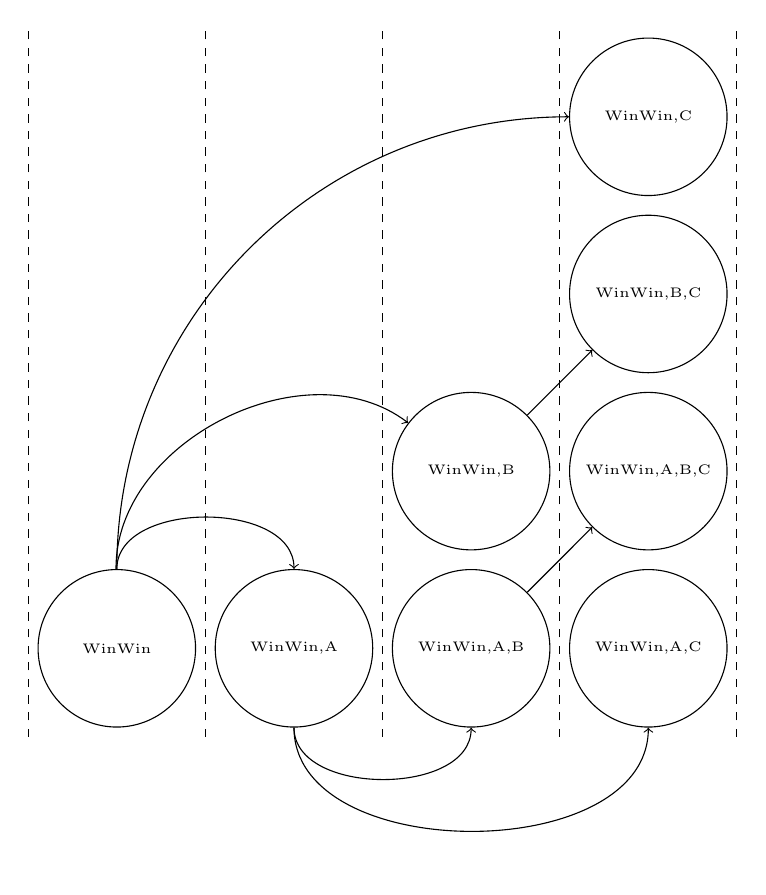
\begin{tikzpicture}[every node/.style={draw,circle, minimum size=2cm}, scale=0.75]
	\node at (0, 0) (W) 	{\tiny WinWin};
	\node at (3, 0) (WA)	{\tiny WinWin,A};
	\node at (6, 0) (WAB)	{\tiny WinWin,A,B};
	\node at (6, 3) (WB)	{\tiny WinWin,B};
	\node at (9, 3) (WABC)	{\tiny WinWin,A,B,C};
	\node at (9, 0) (WAC)	{\tiny WinWin,A,C};
	\node at (9, 6) (WBC)	{\tiny WinWin,B,C};
	\node at (9, 9) (WC)	{\tiny WinWin,C};

	\draw[dashed] (-1.5, -1.5) -- (-1.5, 10.5);
	\draw[dashed] (1.5, -1.5) -- (1.5, 10.5);
	\draw[dashed] (4.5, -1.5) -- (4.5, 10.5);
	\draw[dashed] (7.5, -1.5) -- (7.5, 10.5);
	\draw[dashed] (10.5, -1.5) -- (10.5, 10.5);

	\draw [->] (W) edge[bend left=90] (WA) (W) edge[bend left=64] (WB) (W) edge[bend left = 45] (WC);
	\draw [->] (WA) edge[bend right=90] (WAB) (WA) edge[bend right=90] (WAC);
	\draw [->] (WAB) edge (WABC);
	\draw [->] (WB) edge (WBC);
\end{tikzpicture}
	\caption{Wachstum der Map}
	\label{abb:map}
\end{figure}

\section{Implementierung der Heuristik}
Die Heuristik habe ich innerhalb der BufferedMap implementiert. Nach jeder Leerung des Puffers wird überprüft, ob die maximale Größe der Map überschritten wurde.
Sollte dies der Fall sein, werden niedrigwertige Knoten aus dem Baum gelöscht. Dafür ist nötig, die Knoten nach Wert zu sortieren.

Da die Standardbibliothek eine solche Sortierung nicht vorsieht, musste ich einen eigenen Komparator (Listing \ref{lst:komp}) entwickeln. Dieser Komparator besitzt eine Referenz auf die Map. Beim Vergleich von zwei Mengen lädt der Komparator ihre jeweiligen Werte aus der Map und vergleicht diese. Der Komparator ist so ausgeführt, dass aufsteigend sortiert wird.

Für die eigentliche Sortierung wird das Array über alle Keys, also den Knoten des Baumes, aus der Map extrahiert. Dieses wird dann mithilfe einer parallelen MergeSort-Implementierung sortiert. MergeSort hat den Vorteil das die Laufzeit vorhersehbar ist und somit der Nutzer vor Ablauf geeignete Parameter auswählen kann. Aufgrund der großen Datenmengen und fertigen Implementierung innerhalb der Standardbibiliothek lohnt sich Parallelisierung hier.

Anschließend werden soviele Einträge wie vom Nutzer spezifiziert gelöscht. Um im Nachhinein festzustellen, ob die Heurisitk angewandt wurde wird nach jedem Heuristikdurchlauf ein Zähler erhöht.

Da die Heuristik innerhalb der Datenstruktur implementiert wurde, ist sie für den restlichen Algorithmus transparent und kann gegebenfalls leicht durch eine bessere ersetzt werden.